\section{Introduction to Ethereum}
\label{sec:eth-blockchain}
Open source blockchain networks such as Ethereum and Bitcoin are kits that allow you to set up an economic system in software, complete with account management and a native unit of exchange to pass between accounts. These native units of exchange are called coins, tokens, or cryptocurrencies, but the are no different from tokens in any other system: they are a form of money  that is usable only within that system to simply pay your peers or to run programs on the Ethereum network. 
When you want to make one of these peer-to-peer networks accessible through a web browser, you need to use special software libraries such as Web3\footnote{\url{https://github.com/ethereum/web3.py}},as utilized in this thesis to connect to the Ethereum network \cite[2]{dannen2017introducing}.
The fact that everyone in the world can interact with the same distributed database, given you have internet access and a decent device is favoritable for a fixity storage such as presented in \ref{chapter:fixity_storage} since anyone will be able to confirm if an object has changed over time if given the right resources, such as the transaction hash in which the fixity information of an object was stored on the blockchain. Lets picture an digital archive which releases multiple objects to the public and their respective fixity information on the blockchain, citizens could then validate if the object in question is authentic. Pure trust, that an archive or its stewards did not tamper with the data in their care is therefore not needed anymore.
\section{About the blockchain}
A block is a unit of time that encompasses a certain number of transactions. Inside that period, transaction data is recorded; when the unit of time elapses, the next block begins. The blockchain represents the history of state changes within the network database of the EVM \cite[43]{dannen2017introducing}.
Transactions and state changes in the Ethereum network are segmented into blocks, and then hashed. Each block is verified and validated before the next canonical block can be placed on top of it. In this way, nodes on the network do not need to individually evaluate the trustworthiness of every single block in the history of the Ethereum network, simply to compute the present balances of the accounts on the network. They merely verify that its “parent block” is the most recent canonical block. They do this quickly by looking to see that the new block contains the correct hash of its parents transactions and state. All the blocks strung together, and including the genesis block, an honorific describing the first block the network mined after coming online, are called the blockchain. In some circles, you will hear the blockchain referred to as a distributed ledger or distributed ledger technology (DLT). Ledger is an accurate description, as the chain contains every transaction in the history of the network, making it effectively a giant, balanced book of accounts \cite[55]{dannen2017introducing}. 
\section{Ethereum Virtual Machine}
\label{sec:evm}
The EVMs physical instantiation can not be described in the same way that one might point to a cloud or an ocean wave, but it does exist as one single entity maintained by thousands of connected computers running an Ethereum client \footnote{\url{https://ethereum.org/en/developers/docs/evm/}}.
A virtual machine (VM), in the Ethereum context, is one giant global computer composed of constituent nodes, which are themselves computers too. Generally speaking, a virtual machine is an emulation of a computer system by another computer system. These emulations are based on the same computer architectures as the target of their emulation, but they are usually reproducing that architecture on different hardware than it may have been intended for. Virtual machines can be created with hardware, software, or both. In the case of Ethereum, it is both. Rather than securely network thousands of discrete machines, Ethereum takes the approach of securely operating one very large state machine that can encompass the whole Earth \cite[48]{dannen2017introducing}.
The EVM can run arbitrary computer programs written in the Solidity\footnote{\url{https://github.com/ethereum/solidity}} language. These programs, given a particular input, will always produce the output the same way, with the same underlying state changes. This makes Solidity programs fully deterministic and guaranteed to execute, provided youve paid enough for the transaction. Solidity programs are capable of expressing all tasks accomplishable by computers, making them theoretically Turing complete. That means that the entire distributed network, every node, performs every program executed on the platform \cite[50]{dannen2017introducing}. 
From the perspective of a software developer, the EVM is also a runtime environment for small programs that can be executed by the network. The EVM has its own language, the EVM bytecode, to which smart contracts compile. Solidity, which is a high-level language, is compiled into bytecode and uploaded onto the Ethereum blockchain by using a client application such as truffle\footnote{\url{https://trufflesuite.com/}} or geth\footnote{\url{https://geth.ethereum.org/}} \cite[51]{dannen2017introducing}. 
I have decided to use truffle for my thesis because of its fast and easy way to interact with the Ethereum network and its subnetworks.
\section{Smart Contracts}
Smart contracts are the building blocks of decentralized applications running on the EVM, they are like the concept of classes in conventional object-oriented programming. When developers speak of writing smart contracts, they are typically referring to the practice of writing code in the Solidity language to be executed on the Ethereum network. When the code is executed, units of value may be transferred as easily as data \cite[10]{dannen2017introducing}.
In my thesis, the fixity storage is often referred to as decentralized application (DAPP) which is built with several smart contracts. The smart contract implement in this thesis is further described in Section \ref{sec:implementation}. 

\section{Persistence}
Unlike a centralized server operated by a single company or organization, decentralized storage systems consist of a peer-to-peer network of user-operators who hold a portion of the overall data, creating a resilient file storage sharing system. These can be in a blockchain-based application or any peer-to-peer-based network. Ethereum itself can be used as a decentralized storage system, and it is when it comes to code storage in all the smart contracts. However, when it comes to large amounts of data, that isn't what Ethereum was designed for. The chain is steadily growing and on March 19 2022, the Ethereum chain is at 602.95 GB \footnote{\url{https://ycharts.com/indicators/ethereum_chain_full_sync_data_size}}, which every node on the network needs to be able to store. If the chain were to expand to large amounts of data (say 5TBs) it wouldn't be feasible for all nodes to continue to run. Also, the cost of deploying this much data to Mainnet would be prohibitively expensive due to gas fees \footnote{\url{https://ethereum.org/en/developers/docs/storage/}}.
My proposed solution utilizing pooled testing, presented in Chapter \ref{chapter:pooled_testing}, mitigating the ever increasing chain size of the Ethereum network by reducing the amount of transactions needed to operate the fixity storage.The gas cost of storing a SHA256 value on the blockchain can be read from Table \ref{table:gas-costs}. TODO wie viel gas kostet ein sha256 wort



All transactions in Ethereum are stored on the blockchain, a canonical history of state changes stored on every single Ethereum node \cite[12]{dannen2017introducing}.
Like all databases, a blockchain has a schema: rules define, constrain, and enforce relationships between entities. Motivations to break or alter these relationships can be found across industries, leading to bribery and corruption, and making blockchains trustless qualities even more attractive to business than prior generations of software and networking. In all databases, shared read/write access creates enormous complexity. Machines all over the world may experience varying latency, depending on where the database is physically located, leading to some write operations arriving out of order. This gets even more difficult if several parties are supposed to equally share a database \cite[20]{dannen2017introducing}. 
The nodes go through the block they are process and run any code enclosed within the transactions. Each node does this independently; it is not only highly parallelized, but highly redundant. Despite the high redundany, this is an efficient way to balance a global ledger in a trustworthy way \cite[50]{dannen2017introducing}.
\subsection{Blockchain-based persistence}
This type of persistence is utilized in my thesis, since the fixity information of the archived objects are meant to be persisted for longterm.
For a piece of data to persist forever, Ethereum needs to use a persistence mechanism. For example the persistence mechanism is that the whole chain needs to be accounted for when running a node. New pieces of data get tacked onto the end of the chain, and it continues to grow - requiring every node to replicate all the embedded data. This is known as blockchain-based persistence. The issue with blockchain-based persistence is that the chain could get far too big to upkeep and store all the data feasibly (e.g. many sources estimate the Internet to require over 40 Zetabytes of storage capacity). The blockchain must also have some type of incentive structure. For blockchain-based persistence, there is a payment made to the miner. When the data is added to the chain, the nodes are paid to add the data on \footnote{\url{https://ethereum.org/en/developers/docs/storage/}}.
\subsection{Contract-based persistence}
Contract-based persistence has the intuition that data cannot be replicated by every node and stored forever, and instead must be upkept with contract agreements. These are agreements made with multiple nodes that have promised to hold a piece of data for a period of time. They must be refunded or renewed whenever they run out to keep the data persisted. In most cases, instead of storing all data on-chain, the hash of where the data is located on a chain gets stored. This way, the entire chain doesn't need to scale to keep all of the data \footnote{\url{https://ethereum.org/en/developers/docs/storage/}}.
\section{Test Networks}. 
These networks are not really free of charge, but the ETH token on the respective network is free to get. Although the queue of the free ETH token can be very vast in some cases, e.g. \url{https://faucet.dimensions.network/} this faucet has a waiting queue for over three days until you recieve one ETH token for the ropsten network. Other faucets, a distributer of free ETH test tokens, require social network accounts to verifiy that you are not a bot e.g. \url{https://faucet.paradigm.xyz/} requires a twitter account with at least one tweet and at least 15 retweets before you can request one ETH token. The faucet request are almost all time gated, meaning that you could request ETH only once per day. At small scale, this limitation is no problem for this thesis because persisting around 10 pools on the blockchains require at max 0.002 ETH tokens. The one per day paradigm gets problemeatic for the experiment for the 10.000 objects, which costs about 20 ETH tokens, which means I would have to request tokens fors 20 days straight to perform one experiment on a real live environment such as the ropsten testnetwork. 
There are multiple options to choose from for a testnetwork, from the most prominent networks presented at the official ethereum documentation \footnote{\url{https://ethereum.org/en/developers/docs/networks/}} only the ropsten network implements the proof-of-work algorithm, which means it is the best representation of ethereum to date, and for that reason I decided to utilize the ropsten network in my thesis.
\section{Gas and Fees}
\label{sec:costs}
Gas refers to the unit that measures the amount of computational effort required to execute specific operations on the Ethereum network, this property allows me to calculate the operation cost for the fixity storage without taking the price fluctuation of ETH into account. Since each Ethereum transaction requires computational resources to execute, each transaction requires a fee. Gas refers to the fee required to conduct a transaction on Ethereum successfully.
Gas fees are paid in Ethereum's native currency, ETH (ETH). Gas prices are denoted in gwei, which itself is a denomination of ETH - each gwei is equal to 0.000000001 ETH. For example, instead of saying that your gas costs 0.000000001 ether, you can say your gas costs 1 gwei. The word 'gwei' itself means 'giga-wei', and it is equal to 1,000,000,000 wei. Wei itself is the smallest unit of ETH\footnote{\url{https://ethereum.org/en/developers/docs/gas/}}.
Miners are paid in ETH for mining, and also for running scripts on the network. The cost associated with electricity expenditure of servers running on the Ethereum network is one of the factors that gives ETH, as a cryptocommodity, its intrinsic value—that is, someone paid real money to their electricity company to run their mining machine. Specialized mining rigs, which use arrays of graphics cards to increase their odds of completing a block and getting paid \cite[12]{dannen2017introducing}. 
Mining achieves the consensus required to make valid state changes, and the miners are paid for contributing to the consensus building. This is how ETH and bitcoin are created  \cite[57]{dannen2017introducing}. 
For every instruction the EVM executes, there must be a cost associated, to ensure the system isnt jammed up by useless spam contracts. Every time an instruction executes, an internal counter keeps track of the fees incurred, which are charged to the user. Each time the user initiates a transaction, that users wallet reserves a small portion to pay these fees \cite[58]{dannen2017introducing}. The costs are the driving factor of my thesis where I try to make as less transactions as possible to run a fixity storage on the Ethereum network. 
The fees are dependent on the gas cost of a transaction, gas is a unit of work; it is not a subcurrency, and you can not hold or hoard it. It simply measures how much effort each step of a transaction will be, in computational terms. To be able to pay for gas costs, you simply need to add ETH to your account. You do not have to acquire it separately; there is no gas token. Every operation possible on the EVM has an associated gas cost. Gas costs ensure that computation time on the network is appropriately priced \cite[59]{dannen2017introducing}.
If you send a computationally difficult set of instructions to the EVM, the only person this hurts is you. The work will spend your ether, and stop when the ETH you allocated to the transaction runs out. It has no effect on anyone elses transactions. There is no way to jam up the EVM without paying a lot, in the form of transaction fees, to do it. Scaling is handled in a de facto way through the gas fee system. Miners are free to choose the transactions that pay the highest fee rates, and can also choose the block gas limit collectively. The gas limit determines how much computation can happen (and how much storage can be allocated) per block \cite[60]{dannen2017introducing}. 
\section{Transactions}
An Ethereum transaction refers to an action initiated by an externally-owned account, in other words an account managed by a human, not a contract. For example, if Bob sends Alice 1 ETH, Bob's account must be debited and Alice's must be credited. This state-changing action takes place within a transaction. 
\begin{figure}[h]
    \caption{Illustration of an ethereum transaction \url{https://ethereum.org/en/developers/docs/transactions/}}
    \centering
    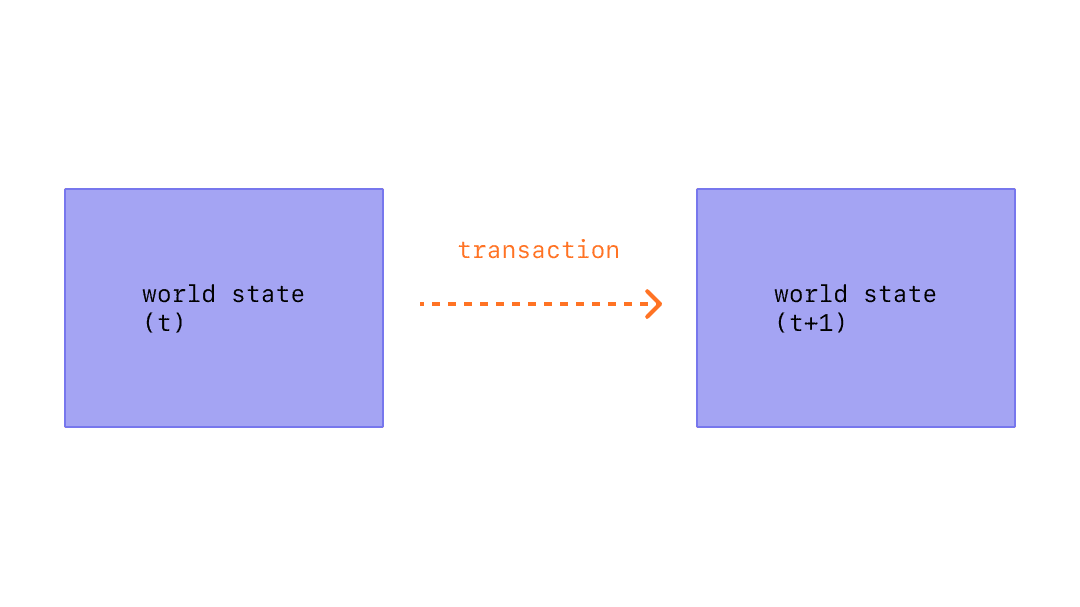
\includegraphics[width=0.5\textwidth]{eth_transaction.png}
\end{figure}
Transactions, which change the state of the EVM, need to be broadcast to the whole network. Any node can broadcast a request for a transaction to be executed on the EVM; after this happens, a miner will execute the transaction and propagate the resulting state change to the rest of the network. \footnote{\url{https://ethereum.org/en/developers/docs/transactions/}}.
Transactions, which do not alter the global state are free of charged and are referred to as Calls. In the source code, as seen in the source code in \ref{lst:fixity-storage}, \textit{getPoolHash(uint32 poolId)} is marked with they keyword view, which means the function itself does not alter the state of the network. Contrary to the function \textit{setPoolHash(uin32 poolId, bytes32 poolHash)} which does alter the networks state and therefore generates cost for the fixity storage. In this thesis, writing actions on the blockchain are often referred to as transactions; and reading actions are reffered to as calls.

TODO Verbatim von ana transaction einfügen, vl von ganache oder etherscan

Transactions come from external accounts, which are usually controlled by human users. It is a way for an external account to submit instructions to the EVM to perform some operation. In other words, it is a way for an external account to get a message into the system. A transaction in the EVM is a cryptographically signed data package storing a message, which tells the EVM to transfer ether, create a new contract, trigger an existing one, or perform some calculation. Contract addresses can be the recipients of transactions, just like users with external accounts \cite[60]{dannen2017introducing}. 
Table \ref{table:gas-costs} presents the gas cost of the most relevant network operations used in this thesis according to the Ethereum yellow paper \cite[27]{wood2014ethereum}.
\begin{center}
    \begin{tabular}{ c c c }\label{table:gas-costs}
     Operation Name & Gas Cost & Description \\ 
     $G_codedeposit$ & 200 & gas cost per bytesize of the compiled bytecode of the smart contract \\  
     $G_txcreate$ & 32000 & create a new smart contract  \\   
     $G_transaction$ & 21000 & retrieve the current balance of an account \\
     $G_txdatanonzero$ & 16 & gas cost per bytesize of the compiled bytecode of the transaction  \\   
     $G_balance$ & 400 & retrieve the current balance of an account 
    \end{tabular}
\end{center}